\documentclass[12pt]{article}
\usepackage[T1]{fontenc}
\usepackage[utf8]{inputenc}
\usepackage{polski}
\usepackage{minted}
\usepackage{geometry}
\usepackage{natbib}
\usepackage{enumitem}
\usepackage{graphicx}
\usepackage{bold-extra}
\usepackage[font=small,labelfont=bf]{caption}
\usepackage{hyperref}
\usepackage{titlesec}
\usepackage{indentfirst}
\hyphenpenalty=10000
\tolerance=1000 \emergencystretch=2em
\titlelabel{\thetitle.\quad}

 \geometry{
     left=23mm,
     top=25mm,
     right=23mm
 }


\def\mydate{\leavevmode\hbox{\twodigits\day.\twodigits\month.\the\year}}
\def\twodigits#1{\ifnum#1<10 0\fi\the#1}

\begin{document}
%titlepage
\thispagestyle{empty}
\begin{center}
\begin{minipage}{0.75\linewidth}
    \centering
    
\includegraphics[width=0.45\linewidth]{agh_logo2.png}
    \par
    \vspace{2cm}
    {\bfseries{\scshape{\Huge  Teoria współbieżności}}}
    \par
    \vspace{2cm}
    {\scshape{\Large Laboratorium 6}}
    \par
    \vspace{0.4cm}
    {\scshape{\Large Problem pięciu filozofów}}
    \par
    \vspace{3cm}

    {\scshape{\Large Albert Gierlach}}\par
    \vspace{1cm}

    {\Large \mydate}
\end{minipage}
\end{center}
\clearpage



\section{Zadanie 1}
Zaimplementowac trywialne rozwiazanie problemu pięciu filozofów z symetrycznymi filozofami. Zaobserwowac problem blokady.

  
\section{Koncept rozwiązania}
Każdy filozof otrzyma dostęp do dwóch widelców - po lewej oraz po prawej stronie. Gdy filozof będzie chciał jeść, to najpierw sięgnie on po lewy widelec, a później po prawy. W programie określiłem liczbę obiadów, którą musi zjeść każdy z filozofów (50 obiadów). Czas myślenia jest trzy razy dłuższy niż czas jedzenia. Zmierzone zostaną czasy, mówiące o tym jak długo każdy z filozofów oczekiwał na dostęp do widelca. Przeprowadzone zostanie 50 powtórzeń, a wynikiem będą uśrednione czasy.

Z racji iż może dojść do zakleszczenia, dodałem czas, po którym wątki zostaną automatycznie zakończone (30 sekund). Czasy z przypadku, w którym nastąpiła blokada nie będą uwzględnione w finalnych uśrednieniach.


\section{Implementacja oraz wyniki}
\begin{minted}[frame=lines,
                framesep=2mm
                ]{java}
class Fork{
    private final Semaphore semaphore = new Semaphore(1);

    public void acquire() throws InterruptedException {
        semaphore.acquire();
    }

    public void release(){
        semaphore.release();
    }
}

class Philosopher extends Thread{
    private static final int EATING_TIME = 30;
    private static final int THINKING_TIME = 90;
    private static final int ITERATIONS = 50;

    private final Fork f1;
    private final Fork f2;
    private final Integer ID;
    private long starvingTime = 0;

    public Philosopher(int i, Fork f1, Fork f2) {
        this.ID = i;
        this.f1 = f1;
        this.f2 = f2;
    }

    @Override
    public void run(){
        for (int i = 0; i < ITERATIONS; i++) {
            think();
            try{
                eat();
            }catch (InterruptedException exception){
                break;
            }
        }
    }

    public void action(Integer time){
        try {
            sleep(time);
        } catch (InterruptedException ignored) {
        }
    }

    public void think(){
//        System.out.println("thinking " + ID);
        action(THINKING_TIME);
    }

    public void eat() throws InterruptedException {
        long before = System.currentTimeMillis();
        f1.acquire();
        f2.acquire();
        long after = System.currentTimeMillis() - before;
        starvingTime += after;
//        System.out.println("eating " + ID);
        action(EATING_TIME);
        f2.release();
        f1.release();
    }

    public long getStarvingTime() {
        return starvingTime;
    }
}

class Main {
    public static Integer PHILOSOPHERS_NUM = 5;

    public static void main(String[] args) {
        var results = new LinkedList<String>();

        var times = testCaseWrapper();
        var stringBuilder = new StringBuilder();
        for(var t : times){
            stringBuilder.append(t);
            stringBuilder.append(",");
        }

        System.out.println(stringBuilder.toString());
        results.add(stringBuilder.toString());

        Path out = Paths.get("philosophers_deadlock.csv");
        try {
            Files.write(out, results, Charset.defaultCharset());
        } catch (IOException e) {
            e.printStackTrace();
        }
    }

    public static long[] testCaseWrapper() {
        var times = new LinkedList<long[]>();

        IntStream.range(0, 50).forEach(i -> {
            var results = testCase();
            results.ifPresent(times::add);
        });

        return Arrays.stream(
                        times
                            .stream()
                            .reduce(new long[PHILOSOPHERS_NUM], (sums, r) -> {
                                IntStream.range(0, PHILOSOPHERS_NUM).forEach(i -> {
                                    sums[i] += r[i];
                                });
                                return sums;
                        }))
                .map(v -> v / times.size())
                .toArray();
    }

    public static Optional<long[]> testCase(){
        var philosophers = new Philosopher[PHILOSOPHERS_NUM];
        var forks = new Fork[philosophers.length];

        IntStream.range(0, PHILOSOPHERS_NUM).forEach(i -> {
            forks[i] = new Fork();
        });

        IntStream.range(0, PHILOSOPHERS_NUM).forEach(i -> {
            philosophers[i] = new Philosopher(i, forks[i], forks[(i+1) % forks.length]);
        });

        var executor = Executors.newFixedThreadPool(5);
        Arrays.stream(philosophers).forEach(executor::submit);
        executor.shutdown();
        boolean finishedNormally = false;
        try {
            finishedNormally = executor.awaitTermination(30, TimeUnit.SECONDS);
        } catch (InterruptedException ignored) {
        }

        if(finishedNormally){
            var results = new long[PHILOSOPHERS_NUM];
            IntStream.range(0, PHILOSOPHERS_NUM).forEach(i -> {
                results[i] = philosophers[i].getStarvingTime();
            });

            return Optional.of(results);
        }

        System.out.println("timeout");
        executor.shutdownNow();
        return Optional.empty();
    }
}
\end{minted}

\newpage
\noindent
Wykonanie programu dało następujące wyniki:
\begin{minted}[frame=lines,
                framesep=2mm
                ]{text}
timeout
396,404,406,409,410,
\end{minted}

\noindent
Po wykonaniu programu stworzono wykres czasów.
\begin{center}
\centering
    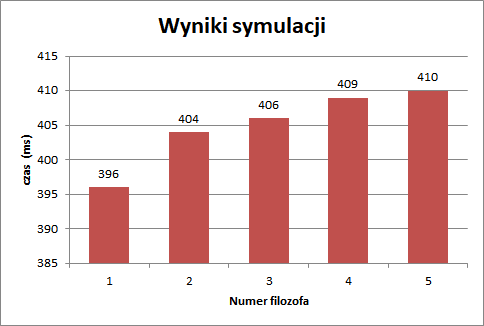
\includegraphics{philosophers_deadlock.png}
    \captionof{figure}{Wyniki symulacji}
\end{center}


\section{Wnioski}
Możemy zauważyć, że oprócz czasów (w milisekundach) pojawiło się słowo \emph{timeout}. Oznacza to, że w jednym przypadku doszło do zakleszczenia. Wykres pokazuje, że czasy oczekiwania na widelce są bardzo zbliżone do siebie. Wynika to z tego, że filozofowie podnoszą widelce w sposób niedeterministyczny.
Warto zauważyc, że zakleszczenie może wystąpić w sytuacji, gdy każdy filozof podniesie jeden widelec po lewej. Wtedy dojdzie do sytuacji, w której każdy czeka na zwolnienie widelca po prawej, ale nigdy to nie nastąpi.



\newpage
\section{Zadanie 2}
Zaimplementowac rozwiazanie problemu pięciu filozofów z widelcami podnoszonymi jednoczesnie. Jaki problem moze tutaj wystapic?
  
\section{Koncept rozwiązania}
W tym wariancie filozof będzie podnosił oba widelce na raz - najpierw lewy, a potem prawy. Jeżeli jeden z widelców będzie zajęty to filozof zrezygnuje z jedzenia (odkładając widelce, jeśli udało mu się jakiś podnieść) i spróbuje ponownie za jakiś czas.

\section{Implementacja oraz wyniki}
\begin{minted}[frame=lines,
                framesep=2mm
                ]{java}
class Fork {
    private final Semaphore semaphore = new Semaphore(1);

    public boolean tryAcquire() {
        return semaphore.tryAcquire();
    }

    public void release() {
        semaphore.release();
    }
}

class Philosopher extends Thread {
    private static final int EATING_TIME = 90;
    private static final int THINKING_TIME = 30;
    private static final int ITERATIONS = 50;

    private final Integer ID;
    private long starvingTime = 0;
    private final Fork left;
    private final Fork right;

    public Philosopher(int i, Fork left, Fork right) {
        this.ID = i;
        this.left = left;
        this.right = right;
    }

    @Override
    public void run() {
        int i = 0;
        while (i < ITERATIONS) {
            think();
            eat();
            i++;
        }
    }

    public void action(Integer time) {
        try {
            sleep(time);
        } catch (InterruptedException ignored) {
        }
    }

    public void think() {
//        System.out.println("thinking " + ID);
        action(THINKING_TIME);
    }

    public void eat() {
        boolean success = false;
        long before = System.currentTimeMillis();

        while (!success) {
            if (left.tryAcquire()) {
                if (right.tryAcquire()) {
                    long after = System.currentTimeMillis() - before;
                    starvingTime += after;

//            System.out.println("eating " + ID);
                    action(EATING_TIME);
                    success = true;

                    right.release();
                }
                left.release();
            }
        }
    }

    public long getStarvingTime() {
        return starvingTime;
    }
}

class Main {
    public static Integer PHILOSOPHERS_NUM = 5;

    public static void main(String[] args) {
        var times = testCase();
        var stringBuilder = new StringBuilder();
        for (var t : times) {
            stringBuilder.append(t);
            stringBuilder.append(",");
        }

        System.out.println(stringBuilder.toString());

        Path out = Paths.get("philosophers_both_forks.csv");
        try {
            Files.writeString(out, stringBuilder.toString(), Charset.defaultCharset());
        } catch (IOException e) {
            e.printStackTrace();
        }
    }

    public static long[] testCase() {
        var philosophers = new Philosopher[PHILOSOPHERS_NUM];
        var forks = new Fork[philosophers.length];

        IntStream.range(0, PHILOSOPHERS_NUM).forEach(i -> {
            forks[i] = new Fork();
        });

        IntStream.range(0, PHILOSOPHERS_NUM).forEach(i -> {
            philosophers[i] = new Philosopher(i, forks[i], forks[(i + 1) % forks.length]);
        });

        var executor = Executors.newFixedThreadPool(5);
        Arrays.stream(philosophers).forEach(executor::submit);
        executor.shutdown();

        try {
            executor.awaitTermination(Long.MAX_VALUE, TimeUnit.SECONDS);
        } catch (InterruptedException ignored) {
        }

        var results = new long[PHILOSOPHERS_NUM];
        IntStream.range(0, PHILOSOPHERS_NUM).forEach(i -> {
            results[i] = philosophers[i].getStarvingTime();
        });

        return results;
    }
}
\end{minted}


\noindent
Po wykonaniu programu stworzono wykres czasów.
\begin{center}
\centering
    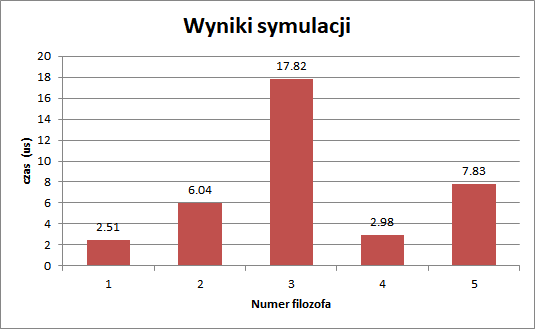
\includegraphics{philosophers_both_forks.png}
    \captionof{figure}{Wyniki symulacji}
\end{center}

\newpage
\section{Wnioski}
Wykres prezentuje dosć wyrównane wyniki, każdy wątek czekał około pięciu sekund. Różnica między najdłuższym czekaniem, a najkrótszym to sekunda. Można stwierdzić więc, że wątek 3 został zagłodzony, ponieważ długo czekał na dostęp do swojej grupy widelców. Zaletą takiej implementacji jest brak możliwości zakleszczenia się, gdyż każdy z filozofów uzyskuje lub czeka na parę widelców, przez co nie może dojść co cyklicznego zakleszczenia, które obserwowaliśmy w zadaniu 1.
Problem występujący w tym wariancie to \emph{zagłodzenie}, czyli wątek, który oczekuje na dostęp do zasobu, będzie długo oczekiwał na jego otrzymanie. 


\section{Zadanie 3}
Zaimplementowac rozwiazanie problemu pięciu filozofów z lokajem.

\section{Koncept rozwiązania}
Do symulacji zostanie wprowadzony lokaj. Będzie on zarządzał dostępem do widelców. Zostanie on zaimplementowany jako semafor zliczający do czterech. Pozwoli to uniknąć zakleszczeń, ponieważ maksymalnie czterech filozofów może na raz prosić od dostęp, czyli gwarantuje to, że ktoś otrzyma dwa widelce.

\section{Implementacja oraz wyniki}

\begin{minted}[frame=lines,
                framesep=2mm
                ]{java}
class Fork {
    private final Semaphore semaphore = new Semaphore(1);

    public void acquire() throws InterruptedException {
        semaphore.acquire();
    }

    public void release() {
        semaphore.release();
    }
}

public class Arbiter {
    private final Semaphore semaphore = new Semaphore(Main.PHILOSOPHERS_NUM-1);

    public void acquireForks() throws InterruptedException {
        semaphore.acquire();
    }

    public void releaseForks(){
        semaphore.release();
    }
}

class Philosopher extends Thread {
    private static final int EATING_TIME = 30;
    private static final int THINKING_TIME = 90;
    private static final int ITERATIONS = 50;

    private final Fork f1;
    private final Fork f2;
    private final Integer ID;
    private long starvingTime = 0;
    private final Arbiter arbiter;

    public Philosopher(int i, Arbiter arbiter, Fork f1, Fork f2) {
        this.ID = i;
        this.f1 = f1;
        this.f2 = f2;
        this.arbiter = arbiter;
    }

    @Override
    public void run() {
        for (int i = 0; i < ITERATIONS; i++) {
            think();
            try {
                eat();
            } catch (InterruptedException exception) {
                break;
            }
        }
    }

    public void action(Integer time) {
        try {
            sleep(time);
        } catch (InterruptedException ignored) {
        }
    }

    public void think() {
//        System.out.println("thinking " + ID);
        action(THINKING_TIME);
    }

    public void eat() throws InterruptedException {
        long before = System.currentTimeMillis();

        arbiter.acquireForks();
        f1.acquire();
        f2.acquire();

        long after = System.currentTimeMillis() - before;
        starvingTime += after;
//        System.out.println("eating " + ID);
        action(EATING_TIME);

        f2.release();
        f1.release();
        arbiter.releaseForks();
    }

    public long getStarvingTime() {
        return starvingTime;
    }
}

class Main {
    public static Integer PHILOSOPHERS_NUM = 5;

    public static void main(String[] args) {
        var times = testCaseWrapper();
        var stringBuilder = new StringBuilder();
        for (var t : times) {
            stringBuilder.append(t);
            stringBuilder.append(",");
        }

        System.out.println(stringBuilder.toString());

        Path out = Paths.get("philosophers_arbiter.csv");
        try {
            Files.writeString(out, stringBuilder.toString(), Charset.defaultCharset());
        } catch (IOException e) {
            e.printStackTrace();
        }
    }

    public static long[] testCaseWrapper() {
        var times = new LinkedList<long[]>();

        IntStream.range(0, 50).forEach(i -> {
            var results = testCase();
            times.add(results);
        });

        return Arrays.stream(
                times
                        .stream()
                        .reduce(new long[PHILOSOPHERS_NUM], (sums, r) -> {
                            IntStream.range(0, PHILOSOPHERS_NUM).forEach(i -> {
                                sums[i] += r[i];
                            });
                            return sums;
                        }))
                .map(v -> v / times.size())
                .toArray();
    }

    public static long[] testCase() {
        var philosophers = new Philosopher[PHILOSOPHERS_NUM];
        var forks = new Fork[philosophers.length];
        var arbiter = new Arbiter();

        IntStream.range(0, PHILOSOPHERS_NUM).forEach(i -> {
            forks[i] = new Fork();
        });

        IntStream.range(0, PHILOSOPHERS_NUM).forEach(i -> {
            philosophers[i] = 
                new Philosopher(i, arbiter, forks[i], forks[(i + 1) % forks.length]);
        });

        var executor = Executors.newFixedThreadPool(5);
        Arrays.stream(philosophers).forEach(executor::submit);
        executor.shutdown();
        try {
            executor.awaitTermination(30, TimeUnit.SECONDS);
        } catch (InterruptedException ignored) {
        }

        var results = new long[PHILOSOPHERS_NUM];
        IntStream.range(0, PHILOSOPHERS_NUM).forEach(i -> {
            results[i] = philosophers[i].getStarvingTime();
        });
        return results;
    }
}

\end{minted}


Po wykonaniu programu stworzono wykres czasów.
\begin{center}
\centering
    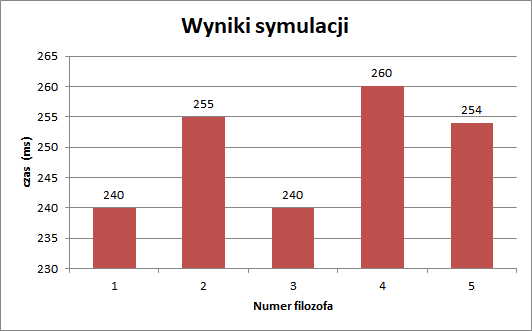
\includegraphics{philosophers_arbiter.png}
    \captionof{figure}{Wyniki symulacji}
\end{center}


\section{Wnioski}
Wykres przedstawia sumaryczny czas spędzony na oczekiwaniu na dostęp do widelców przez każdego filozofa. Wyniki są zbliżone do siebie, a różnice są na tyle niewielkie, że można stwierdzić, że dostęp do widelców był przydzielany sprawiedliwie. W tym wariancie nie dochodzi do zakleszczenia, ponieważ mamy lokaja, który gwarantuje, że jeden z pięciu filozofów będzie mógł użyć widelców. Rozwiązanie jest wydajniejsze od wariantu przedstawionego w zadaniu pierwszym. Czasy oczekiwań spadły o około 50\%.

\newpage
\section{Bibliografia}
\begin{itemize}
    \item \url{http://wazniak.mimuw.edu.pl/index.php?title=Programowanie_wsp%C3%B3%C5%82bie%C5%BCne_i_rozproszone/PWR_Wyk%C5%82ad_9}
    \item \url{https://en.wikipedia.org/wiki/Dining_philosophers_problem}
    \item \url{https://ccl.northwestern.edu/netlogo/models/DiningPhilosophers}
    \item \url{https://www.prismmodelchecker.org/tutorial/phil.php}
    \item \url{https://pages.mtu.edu/~shene/NSF-3/e-Book/MUTEX/TM-example-philos-1.html}

\end{itemize}

\end{document}
